\documentclass{main}

% mise en place du glossaire
%\setglossarystyle{altlist} % apparence du glossaire
%\makenoidxglossaries % génération du glossaire
%\newglossaryentry{} {
    name=,
    description=
}
 % appel du fichier contenant le glossaire

\begin{document}

\makeatletter
\patchcmd{\ttlh@hang}{\parindent\z@}{\parindent\z@\leavevmode}{}{}
\patchcmd{\ttlh@hang}{\noindent}{}{}{}
\makeatother

\pagenumbering{roman}

%\maketitle

%définition du template du document
\renewcommand{\baselinestretch}{1.0}\normalsize
\newcommand{\itab}[1]{\hspace{0em}\rlap{#1}}
\newcommand{\tab}[1]{\hspace{.2\textwidth}\rlap{#1}}
\renewcommand{\bibname}{Bibliography} % définir le titre de la bibliographie
\renewcommand{\contentsname}{Table of Contents}

%\insertAntiPlagiarismAgreement{Warnet, Nicolas}{31415793}

\cleardoublepage

%\makesecondtitle

\section*{Acknowledging} % l'étoile permet de ne pas numéroter sur la toc
I wish to thank David Ritchie and Bernard Maigret who trusted me to work on
this project and followed me throughout my internship.
  I would also like thank Olivier Devillers for his classes
  on the Delaunay triangulations and his explanations regarding the CGAL library.
   Finally, it is necessary for me to thank all the Capsid team for having facilitated my
    integration in the institute as well as all of the INRIA of Nancy.


%table des matières
\renewcommand{\baselinestretch}{0.5}\normalsize
\tableofcontents
\renewcommand{\baselinestretch}{1.0}\normalsize
\cleardoublepage

\pagenumbering{arabic}
\setcounter{page}{1}

%% INTRODUCTION
\chapter*{Introduction}
\addcontentsline{toc}{chapter}{Introduction}

  L'INRIA (Institut National de Recherche en Informatique et en Automatique) est un
  institut français public de recherche en informatique et en mathématiques. Fondé
  en 1967, l'INRIA compte 2600 collaborateurs rassemblés sur différents sites en
  France dont Nancy. Au sein de ce centre, l'équipe CAPSID développe des algorithmes
  et des logiciels permettant d'étudier des phénomènes et systèmes biologiques
  d'un point de vue structurel, grâce notamment à la modélisation 3D. J'ai effectué
  mon stage au sein de cette équipe sous la tutelle de Dave Ritchie qui en est le
  directeur.

  Supervisé par Dave Ritchie et Bernard Maigret, ce projet a pour objectif de
  modéliser l'interface de contact entre deux protéines. Les propriétés de l'interface
  peuvent en effet donner de nombreuses informations sur les interactions entre
  des protéines. Ceci sert notamment en biologie et en recherche médicinale pour
  le développement de nouveaux médicaments.
  Le projet se déroule également en partenariat avec l'équipe de recherche Vegas, et
  notamment Olivier Devillers, qui a participé à l'imlémentation de
  la librairie d'algorithme de calcul géométrique CGAL (Computational Geometry
  Algorithms Library).

  Cette librairie va permettre, grâce aux nombreuses fonctionnalités qu'elle offre,
  d'améliorer et d'accélerer le développement de la méthode choisie pour le projet.
  Nous détaillerons dans ce rapport la méthode théorique retenue pour approximer l'interface
  entre les protéines : la triangulation de Delaunay et le diagramme de Voronoï. Nous
  expliquerons également comment les structures fournies par CGAL sont utilisées lors
  du développement logiciels en détaillant certaines parties cruciales de l'implémentation.
  Enfin, nous verrons comment les résultats obtenus (et les difficultés rencontrées)
  permettentt d'envisager des perspectives d'avenir pour ce projet.

%\cleardoublepage

\chapter{Méthode + Théorie}

\section{Structure d'une protéine et d'un complexe}

L'objectif du projet étant de modéliser l'interface de contact entre deux protéines,
il est important de comprendre la structure d'une protéine. Nous verrons également
comment sont stockées ces structures, grâce au fichiers \textit{.pdb}.

\subsection*{Structure}

Les protéines sont des molécules biologiques présentes dans toutes les cellules vivantes.
Elles sont constituées d'un enchaînement d'acides aminés \cite{Prot}.
Les protéines assurent diverses fonctions au sein de la cellule vivante et dans les tissus.
Elles peuvent avoir un rôle enzymatique, structurel, permettre la mobilité des molécules, la
régulation de l'expression génétique ou encore transmettre des signaux cellulaires.
Les chaînes protéiques constituant les protéines sont synthétisées dans la cellule. Le
matériel génétique de la cellule détermine l'ordre d'enchaînement des acides aminés.
Les protéines adoptent alors une structure en trois dimensions qui leur permet d'assurer
 leur fonction biologique. Les protéines peuvent interagir ensemble afin d'assurer certaines
fonctions biologiques. Ces interactions forment des complexes protéiques. Les structures
 des protéines et leurs interactions sont particulièrement utilisées en chimie médicinale.
L'étude des surfaces et des espaces disponibles peut guider la recherche d'un nouveau
médicament. La cristallographie est utilisée pour étudier la structure des protéines à
l'échelle atomique. Elle s'appuie sur le phénomène physique de diffraction des ondes
électromagnétiques (rayons X).

Le complexe que nous étudions dans ce projet est l'interaction entre
deux protéines. La structure de ce complexe peut être analysée en étudiant l'interface
entre les deux protéines le composant. On comprend dès lors que modéliser cette interface
pour la visualiser peut avoir une importance cruciale en recherche biologique et médicinale.

\subsection*{Fichier de stockage}

Les données utilisables d'une protéine (ou d'un complexe) sont stockées grâce aux
fichiers \textit{.pdb} (voir figure \ref{fig::pdb_file}). Ces fichiers, leur lecture et l'interprétation des données
qu'ils contiennent, sont essentiels à l'observation des protéines. En effet, chaque
ligne, exceptée la première, correspond à un atome composant la protéine étudiée.
Ces lignes contiennent des informations telles que la chaîne à laquelle appartient
l'atome, son acide aminé ou ses coordonnées dans l'espace (en $\si{\angstrom}$).

\begin{figure}[ht]
  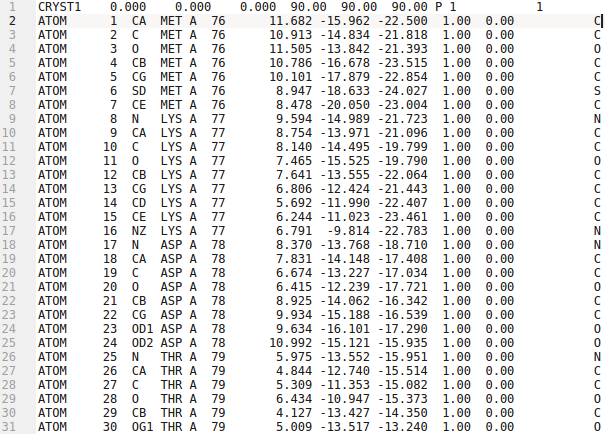
\includegraphics[width=\textwidth]{figures/pdb_example.png}
  \caption{Exemple de fichier .pdb}
  \label{fig::pdb_file}
\end{figure}

Dans la suite du projet, nous considérerons que les atomes sont des points de l'espace
de masses identiques. Dans un premier temps, les coordonnées des atomes seront extraites.
Le nuage de point obtenu constitue la base sur laquelle la méthode de détermination
de l'interface va s'appuyer. Il est donc crucial d'obtenir du fichier \textit{.pdb} un jeu
de données valide et utilisable par le programme implémenté ensuite. Nous verrons également
que d'autres informations, telles que la chaîne (A ou B, colonne 5 de la figure
\ref{fig::pdb_file}), jouent un rôle prépondérant dans le bon fonctionnement du
programme. L'objectif est donc d'extraire un nuage de points cohérent (modélisant
le complexe), pour lui appliquer la triangulation de Delaunay.



\section{Triangulation de Delaunay}

Une protéine est donc représentée comme un nuage de points où chacun de ces points
représente un atome de la protéine. Dans le but d'optimiser les temps de parcours dans
ce nuage de points et de modéliser l'interface entre les deux protéines,
 on utilise la triangulation de Delaunay \cite{Triangulation}.

 Cette triangulation est unique et peut être expliquée de la manière suivante :
 chaque cercle circonscrit à un triangle du nuage de point ne contient que les points
 dudit triangle (voir figure \ref{fig::explication_delaunay}).
 Nous expliquerons dans un premier
 temps la méthode pour déterminer l'interface en deux dimensions avant de la transposer à la
 dimension 3.

\begin{figure}[ht]
\centering
  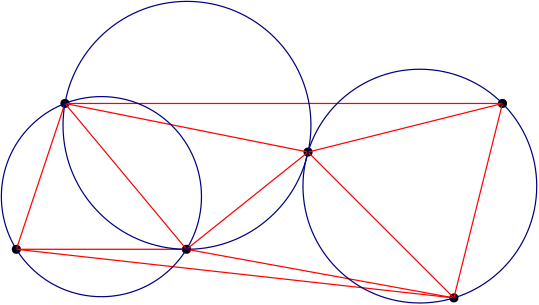
\includegraphics[width=\textwidth]{figures/explication_delaunay.png}
  \caption{Triangulation de Delaunay}
  \label{fig::explication_delaunay}
\end{figure}

\subsection*{Dimension 2}

Il faut appliquer cette triangulation au complexe dont on veut déterminer l'interface, c'est-à dire
aux points donnés par les coordonnées des atomes qui composent le complexe
(voir figure \ref{fig::delaunay_tr}). Les protéines du complexe sont différenciées
par leur couleur (rouge et bleu) sur le schéma. Nous sélectionnons alors la partie utile de
cette triangulation (voir figure \ref{fig::delaunay_reduced}) : nous ne gardons que
les triangles qui contiennent au moins un point à l'interface.
Un point est à l'interface s'il appartient à un triangle contenant au moins un point
de chaque protéine. Le fait de réduire la taille de la triangulation sera utile par la suite
pour accélérer les temps de traitement et de récupération de données concernant l'interface.



\begin{figure}[ht]
\centering
\begin{subfigure}{0.4\textwidth}
  \centering
  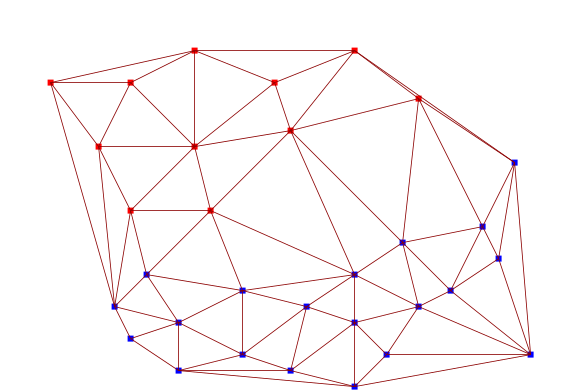
\includegraphics[width=\textwidth]{figures/delaunay.png}
  \caption{Triangulation de Delaunay}
  \label{fig::delaunay_tr}
\end{subfigure}%
\begin{subfigure}{0.2\textwidth}
  \centering
  $\Longrightarrow$
\end{subfigure}%
\begin{subfigure}{0.4\textwidth}
  \centering
  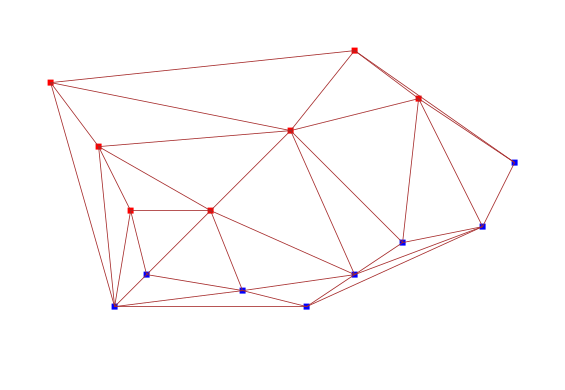
\includegraphics[width=\textwidth]{figures/delaunay_reduced.png}
  \caption{Triangulation réduite}
  \label{fig::delaunay_reduced}
\end{subfigure}
\caption{Réduction d'une triangulation}
\label{fig::delaunays}
\end{figure}

Nous nous intéressons maintenant à la détermination de l'interface, proprement dite.
En ne gardant que les arêtes utiles (voir figure \ref{fig::delaunays_process_1}),
c'est-à-dire celles reliant deux points appartenant
à deux protéines différentes, nous pouvons approximer l'interface de contact grâce
au diagramme de Voronoï.

\begin{figure}[ht]
\centering
\begin{subfigure}{0.45\textwidth}
  \centering
  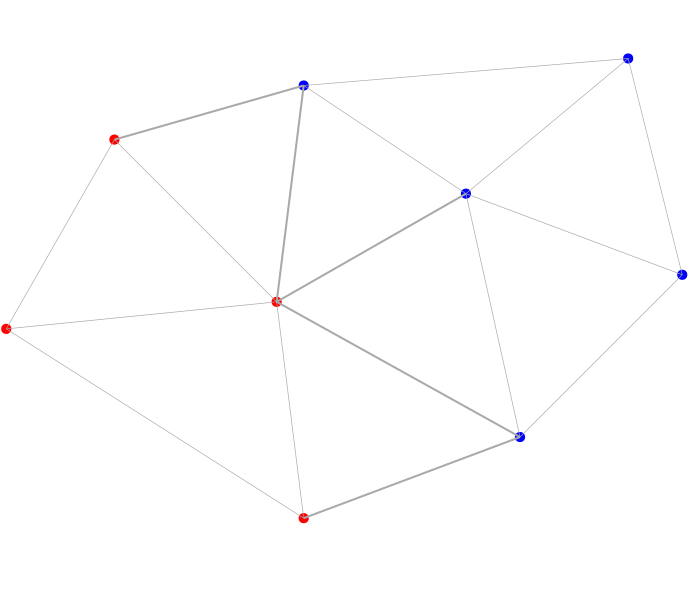
\includegraphics[width=\textwidth]{figures/process_d_1.png}
  \caption{Triangulation de Delaunay}
  \label{fig::process_d_1}
\end{subfigure}%
\begin{subfigure}{0.1\textwidth}
  \centering
  $\Longrightarrow$
\end{subfigure}%
\begin{subfigure}{0.45\textwidth}
  \centering
  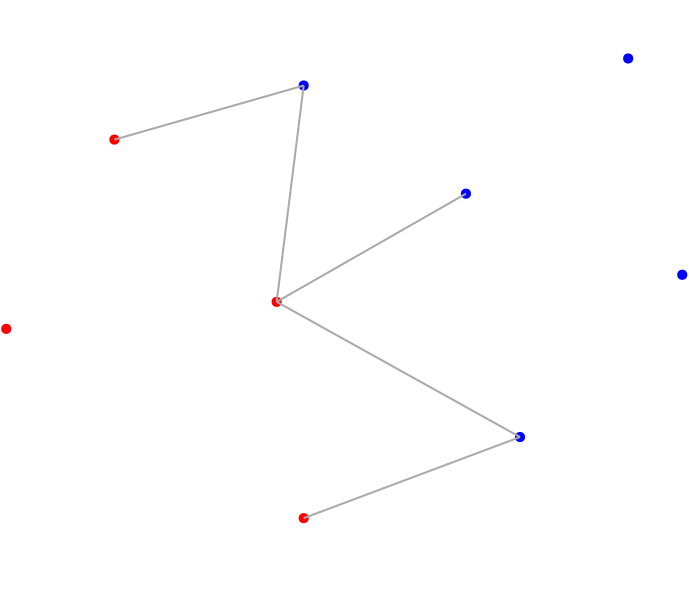
\includegraphics[width=\textwidth]{figures/process_d_2.png}
  \caption{Arêtes à l'interface}
  \label{fig::process_d_2}
\end{subfigure}
\caption{Triangulations et zone utile}
\label{fig::delaunays_process_1}
\end{figure}


Ce diagramme est le dual de la triangulation de Delaunay. Il est representé par les
médiatrices des segments qui constitue la triangulation.
 Il contient donc l'ensemble des points à
égale distance des points de la triangulation (voir figure \ref{fig::process_d_3}).
On ne garde que les parties du diagramme de Voronoï qui correspondent aux arêtes sélectionnées
précédemment, c'est-à-dire les segments du diagramme de Voronoï qui intersectent
avec les arêtes de la triangulation de Delaunay (voir figure \ref{fig::process_d_4}).
Nous obtenons alors une droite par morceaux
qui approxime l'interface de contact en dimension 2.

\begin{figure}[ht]
\centering
\begin{subfigure}{0.45\textwidth}
  \centering
  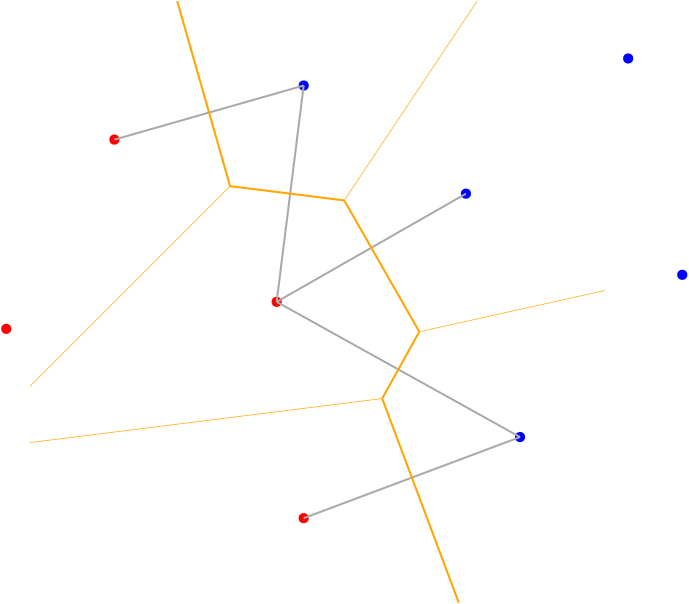
\includegraphics[width=\textwidth]{figures/process_d_3.png}
  \caption{Diagramme de Voronoï}
  \label{fig::process_d_3}
\end{subfigure}%
\begin{subfigure}{0.1\textwidth}
  \centering
  $\Longrightarrow$
\end{subfigure}%
\begin{subfigure}{0.45\textwidth}
  \centering
  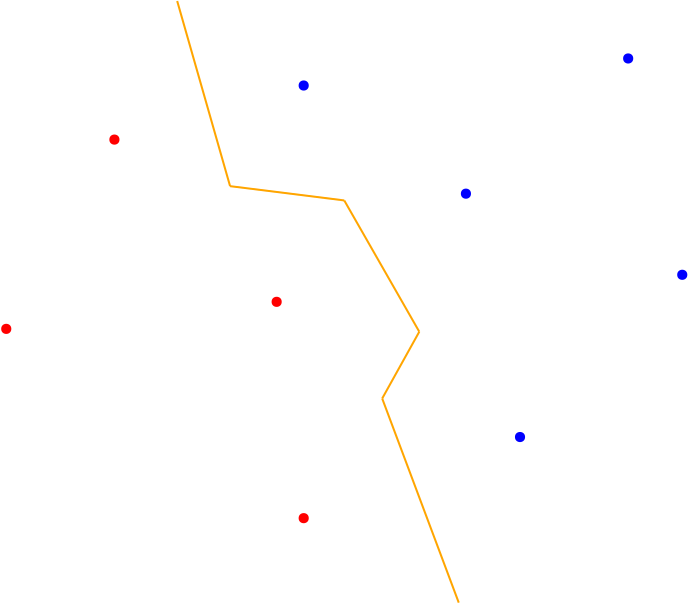
\includegraphics[width=\textwidth]{figures/process_d_4.png}
  \caption{Interface}
  \label{fig::process_d_4}
\end{subfigure}
\caption{Recherche de la surface de contact}
\label{fig::delaunays_process_2}
\end{figure}


\subsection*{Dimension 3}

Si nous transposons la méthode vue ci-dessus en dimension 3, les triangles formés
par les points deviennent des tetrahèdres sur lesquels nous travaillerons pour vérifier
les zones utiles au calcul de l'interface. De la même manière, un tétrahèdre sera considéré
à l'interface s'il contient au moins un atome de chaque protéine.
De plus, le dual d'une arête devient une surface entourant cette arête (voir figure
 \ref{fig::dual_3d}). En rassemblant ces morceaux
de surface, nous obtenons une surface en trois dimensions qui modélise la surface
de contact entre les deux protéines du complexe étudié.

\begin{figure}[ht]
\centering
  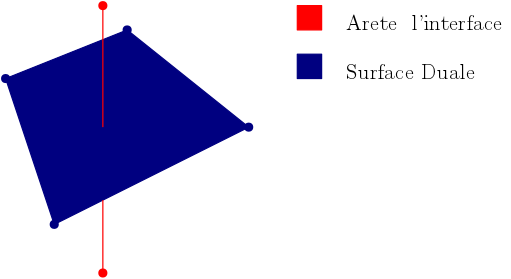
\includegraphics[width=\textwidth]{figures/dual_3d.png}
  \caption{Dual d'une arête en Dimension 3}
  \label{fig::dual_3d}
\end{figure}

La triangulation en trois dimensions d'un nuage de points correspondants aux atomes
d'un complexe donne la figure \ref{fig::delaunays_3d}.

\begin{figure}[ht]
\centering
\begin{subfigure}{0.45\textwidth}
  \centering
  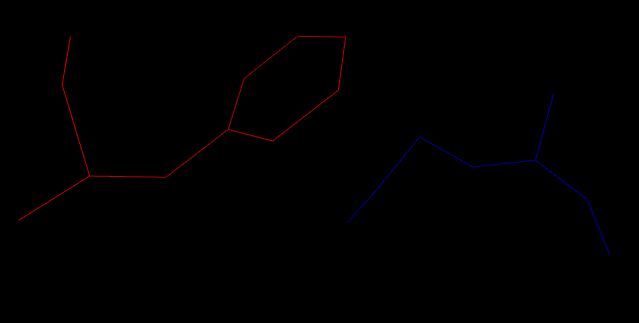
\includegraphics[width=\textwidth]{figures/small_prot.png}
  \caption{Partie d'un complexe}
  \label{fig::small_prot}
\end{subfigure}%
\begin{subfigure}{0.1\textwidth}
  \centering
  $\Longrightarrow$
\end{subfigure}%
\begin{subfigure}{0.45\textwidth}
  \centering
  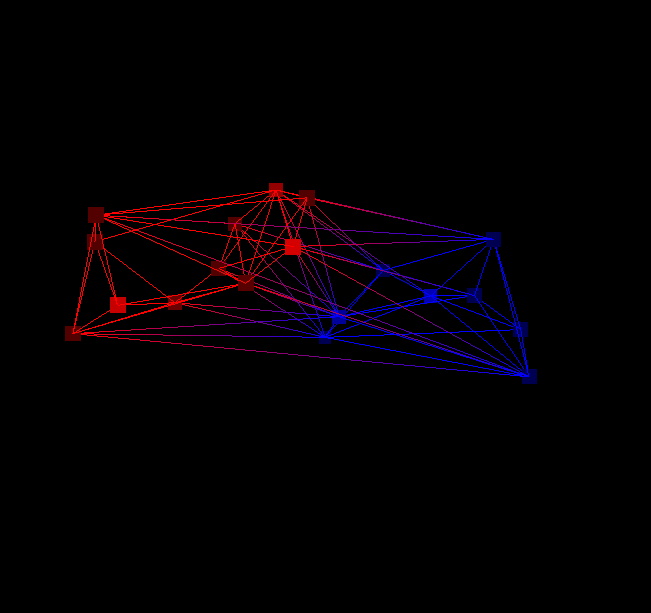
\includegraphics[width=\textwidth]{figures/3d_triangulation04.png}
  \caption{Triangulation}
  \label{fig::prot_delaunay}
\end{subfigure}
\caption{Triangulation 3D d'un complexe}
\label{fig::delaunays_3d}
\end{figure}

\section{CGAL}

Pour développer la méthode vue précédemment, nous avons choisi d'utiliser CGAL
(Computational Geometry Algorithms Library) \cite{CGAL}.
CGAL est un projet logiciel qui fournit un accès libre à de nombreux algorithmes géométriques
efficaces et fiables sous forme d'une bibliothèque C++. CGAL est utilisé dans des
domaines divers ayant besoin de calcul géométrique, tels que des systèmes
d'information géographiques, la conception assistée par ordinateur, la biologie
moléculaire, l'imagerie médicale, l'infographie et la robotique.

Nous nous sommes particulièrement intéressés à une partie de CGAL qui permet le
stockage de nuages de points sous forme de triangulations de Delaunay. L'avantage
de cette bibliothèque réside dans les structures et les méthodes accélérant les différentes
étapes du calcul de l'interface entre deux protéines.

\subsection*{Structures}


En effet, CGAL comprend notamment une classe (que l'on peut voir comme une structure)
\textit{Delaunay\_Triangulation\_3},
permettant de calculer et de stocker une triangulation de Delaunay depuis de simples
tableaux (\textit{C++ Arrays}) listant des points dans l'espace. Pour mieux, comprendre
l'implémentation réalisée durant ce projet, il est important de préciser la structure des tétrahèdres
composant une trianguation de Delaunay (voir figure \ref{fig::tetrahedron_cgal}).

\begin{figure}[ht]
\centering
  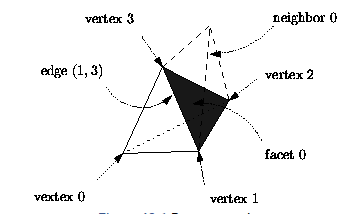
\includegraphics[width=0.5\textwidth]{figures/tetrahedron_cgal.png}
  \caption{Structure d'un tetrahèdre dans CGAL \cite{CGAL}}
  \label{fig::tetrahedron_cgal}
\end{figure}

Un tétrahèdre est représenté par quatre entités :
\begin{itemize}
  \item Vertex (sommet) : contient un point (coordonnées 3D)
  \item Cell (cellule) : un tétrahèdre qui donne accès à quatre sommets et quatre cellules adjacentes (les
  cellules qui ont une face commune avec la cellule courante)
  \item Edge (arête) : une arête contenant deux sommet ordonnés (l'arête va d'un point
  à un autre avec un sens établi) et une cellule
  \item Facet (face) : une face stockée grâce à une cellule et au sommet qui lui
  est opposé dans cette cellule
\end{itemize}

Il est important de comprendre la structure mise en place dans \gls{cgal} car il sera
nécessaire d'accéder aux différentes parties d'un tétrahèdre. Par exemple, lorsque
nous travaillons sur les arêtes pour rechercher l'interface, nous avons besoin de
connaître les sommets qui la composent.

Il existe également une seconde strucure de données, \textit{Polyhedron}, qui sera
utilisée pour stocker la surface. Cette classe permet de travailler sur des surfaces
en trois dimensions c'est-à-dire que les morceaux de cette surface sont en deux dimensions.
Le fonctionnement est sensiblement identique à la classe \textit{Delaunay\_Triangulation\_3}.
En effet, chaque polygone est également composé d'arêtes et de sommets auxquels on peut
accéder pour en récupérer les informations.

La compréhension des structures fournies par CGAL constitue donc une partie fondamentale du
projet. En effet la maîtrise des accesseurs (c'est-à-dire les méthodes qui permettent
d'accéder à chaque entité composant un térahèdre) est cruciale afin d'optimiser les parcours
dans les nuages de points via les itérateurs.





\subsection*{Itérateurs}

Les itérateurs sont une généralisation de pointeurs qui permettent de travailler sur
différentes structures de données. L'avantage est qu'ils sont liés aux différentes entités
qui composent un tétrahèdre. On peut comparer l'utilisation d'un itérateur à une boucle
\textit{for} dont l'ordre de parcours a été choisi au préalable afin d'optimiser
le temps de parcours.
Il existe des itérateurs permettant de parcourir une triangulation de Delaunay
selon chacune des entités formant celle-ci : vertice, arête, face, cellule. Quelle
que soit l'entité utilisée, il est possible d'accéder aux trois autres entités et
aux données qu'elles contiennent. Les itérateurs fonctionnent dans CGAL grâce aux
\textit{Handles}. Celles-ci sont des références indirectes qui fonctionnent sensiblement
comme des pointeurs. Lorsqu'on itère sur un des types composant les tétrahèdres, une
\textit{Handle} vers le type concerné est renvoyée. Par exemple, pour une itération sur des
vertices, on peut accéder à l'indice stocké dans \textit{info()} par la commande
fournie en figure \ref{fig::access_it}.

\begin{figure}[ht]
\centering
  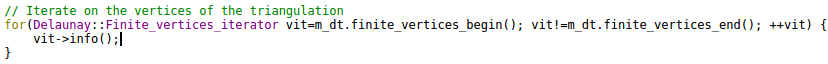
\includegraphics[width=\textwidth]{figures/access_it.png}
  \caption{Utilisation d'un itérateur}
  \label{fig::access_it}
\end{figure}


Il existe également des circulateurs qui, bien que semblables aux itérateurs par le fait
qu'ils parcourent des structures de données, fonctionnent différemment. Comme leur nom
l'indique, ils permettent de "tourner" autour d'une entité. Par exemple ils peuvent
servir à parcourir toutes les cellules adjacentes d'une cellule donnée. Ils s'utilisent
sous la forme d'une boucle \textit{do...while} (voir figure \ref{fig::circ_ex}).
\begin{figure}[ht]
\centering
  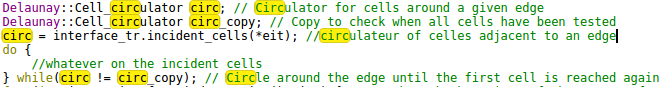
\includegraphics[width=\textwidth]{figures/circ_ex.png}
  \caption{Utilisation d'un circulateur}
  \label{fig::circ_ex}
\end{figure}
 Le circulateur est incrémenté à chaque
passage dans la boucle jusqu'à ce qu'il soit revenu à son point de départ. Il aura alors
effectué un "tour" complet autour de l'entité de notre choix.


Nous verrons, lors de l'implémentation, qu'un bon usage des circulateurs, et plus encore des itérateurs,
est absolument crucial pour l'optimisation des temps de parcours et la validité
des résultats obtenus. Ils permettent également de rendre le code plus générique.

Nous verrons également comment la méthode théorique a été implémentée grâce en partie à CGAL
dans la suite de notre projet.


\chapter{Développement Logiciel}

Dans cette partie, expliquerons le développement du programme en différentes étapes :
l'architecture du programme, la récupération des données, la construction de la surface
et l'affichage (voir figure \ref{fig::flow_chart}).

\begin{figure}[ht]
\centering
  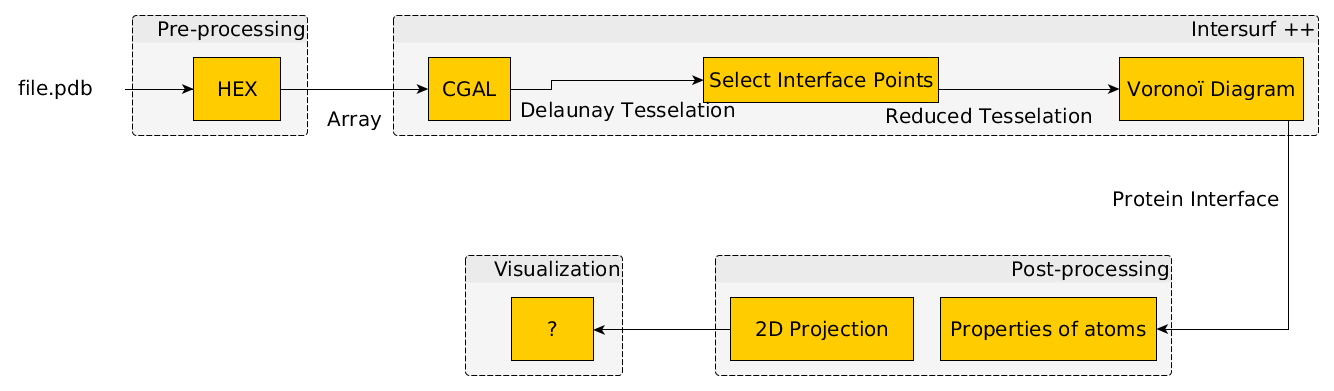
\includegraphics[width=\textwidth]{figures/flow_chart.png}
  \caption{Flow chart du programme}
  \label{fig::flow_chart}
\end{figure}

\section{Architecture Logicielle}
\begin{itemize}
  \item C / C++ / Libraries
  \item Compilation Cmake
\end{itemize}
Les différentes étapes


\section{Récupération de données + stockage}
\begin{itemize}
  \item .pdb files + pdb reader
  \item Tableau et méthode de stockage (C++ structures)
  \item CGAL structures : Delaunay + Polyhedron
\end{itemize}

Le point de départ du projet est de lire un fichier \textit{.pdb} et de le stocker
de manière à créer les structures fournies par CGAL. Nous avons utilisé une partie du programme
\textbf{Hex} développé en C par David Ritchie qui permet de \textit{parser} le fichier
\textit{.pdb} pour récupérer les données utiles du complexe étudié. Ces informations constituent
la référence utilisée lors de la construction de l'interface lorsque des détails
sur les atomes (chaîne, etc.) doivent êre connus. La fonction utilisée pour cela
renvoie un pointeur vers un tableau recensant toutes les informations utiles, c'est-à-dire
une image du fichier \textit{.pdb} que nous appellerons \textit{Image pdb} (voir
figure \ref{fig::read_pdb}).

\begin{figure}[ht]
\centering
  
\includegraphics[width=\textwidth]{figures/pdb_image.png}
  \caption{Récupération des données du fichier \textit{.pdb}}
  \label{fig::read_pdb}
\end{figure}

Pour créer une structure de Delaunay, CGAL prend normalement une liste de points stockée
sous forme de tableau. Cependant, utiliser cette méthode simple ne premettrait pas d'accéder aux
informations contenues dans le fichier \textit{.pdb}. En effet, chaque vertice (point), de la
triangulation de Delaunay doit être indexé de manière à retrouver les informations voulues dans la
liste d'atome fournie par le fichier de départ. Les index doivent donc être choisis
au moment de la lecture de l'\textit{Image pdb} pour correspondre à la place de l'atome
dans le tableau.
Il existe deux méthodes pour insérer un index à une variable de type Vertex dans CGAL :
\begin{itemize}
  \item on modifie la classe Vertex en ajoutant un attribut
  \item on utilise une classe différente fournie par CGAL
\end{itemize}
Nous avons choisi d'utiliser la seconde méthode (voir figure \ref{fig::vertex_base}) pour
sa simplicité. Lors de l'instanciation, cette classe prend notamment en paramètre
\textit{template} un type qui de variable qui sera accessible comme l'attribut \textit{info()}.

\begin{figure}[ht]
\centering
  
\includegraphics[width=0.8\textwidth]{figures/vertex_base.png}
  \caption{Déclaration de la classe \textit{Vertex\_base\_with\_info}}
  \label{fig::vertex_base}
\end{figure}

Le type de l'index est donc un entier positif qui fera partie de la structure Delaunay
et sera accessible lors du parcours de ces structures. Cependant, la structure de Delaunay
requiert l'ajout d'un index lors de son instanciation. Un vecteur de paires contenant
un point 3D et une variable du type de l'attribut \textit{info()} (voir figure
\ref{fig::vector_atom_index}) convient.

\begin{figure}[ht]
\centering
  
\includegraphics[width=\textwidth]{figures/vector_atom_index.png}
  \caption{Déclaration du vecteur contenant les atomes et leurs index}
  \label{fig::vector_atom_index}
\end{figure}

La fonction complète permettant d'écrire un fichier\textit{.pdb} dans une structure
\textit{CGAL::Delaunay} est disponible en annexe (voir figure \ref{fig::read_pdb}).
On remarque la présence de la \textit{map} C++ \textit{is\_interface}
(voir figure \ref{fig::is_interface}) qui sera utilisée par la suite
pour sélectionner les tétrahèdres présents à l'interface (voir figure \ref{fig::delaunays}).

\begin{figure}[ht]
\centering
  
\includegraphics[width=0.5\textwidth]{figures/is_interface.png}
  \caption{Déclaration de la map is\_interface}
  \label{fig::is_interface}
\end{figure}

\section{Construction de la surface}
\begin{itemize}
  \item Tesselation $\to$ Arêtes à l'interface $\to$ Dual (Surface)
  \item Index + Informations : Lien entre le .pdb (Chaîne, Atome, etc.) et les points de la surface
  \item smoothing
\end{itemize}

Lorsque les strucures de Delaunay ont été créées, il devient possible de calculer l'interface
entre les deux protéines du complexe, ce qui constitue la partie centrale du projet.
En implémentant la méthode vue dans la partie Triangulation de Delaunay, nous pouvons générer
une surface qui pourra être affichée. Cette surface est un regroupement de polyhèdres
de nombre de côtés variable.



Dans la première partie de l'implémentation, nous stockons la surface dans \textit{vecteur}
(\textit{all\_faces\_indexes})
et une \textit{map} (\textit{surf\_points}) (voir figure \ref{fig::init_surf_vector}) qui permettent de garder
en mémoire les coordonnées des points
et les indices permettant d'afficher les faces. La \textit{map} recense tous les points
de la surface une fois, c'est-à-dire que les points utilisés dans différentes face de la surface
ne sont présent qu'une seule fois dans la map. Cela permet de réduire considérablement
la quantité de données et d'accélerer l'affichage. A chaque point de la map correspond
un indice initialisé à 0 et qui sera mis à jour lors de l'écriture des fichiers utilisés
pour l'affichage. Ensuite, le \textit{vecteur} regroupe toutes les faces de la surface
sous forme de vecteurs de point 3D. Le vecteur \textit{all\_faces\_indexes} contiendra
donc autant de vecteurs que le nombre de faces de la surface.


\begin{figure}[ht]
\centering
  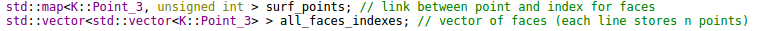
\includegraphics[width=\textwidth]{figures/init_surf_vect.png}
  \caption{Déclaration des vecteurs stockant la surface}
  \label{fig::init_surf_vector}
\end{figure}

Nous allons maintenant détailler les différentes parties de la fonction écrite pour
le calcul de l'interface (\textit{calculateInterface()}) qui est disponible en
annexe (voir figure \ref{fig::calculate_interface}).

Dans un premier temps, nous utilisons un itérateur fourni par CGAL pour parcourir
les arêtes de la triangulation (voir figure \ref{fig::iter_edges}).
\begin{figure}[ht]
\centering
  
\includegraphics[width=\textwidth]{figures/iter_edges.png}
  \caption{Itération sur les arêtes}
  \label{fig::iter_edges}
\end{figure}
Dans cette itération, on vérifie pour chaque arête si elle est à l'interface, c'est-à-dire
si elle possède un atome de chaque chaîne. Pour cela, nous nous référons à l'\textit{Image pdb}
grâce à l'indice stocké dans l'attribut \textit{info()} de chaque vertice. Il est possible
d'accéder à la valeur de la chaîne (A ou B) avec la commande en figure \ref{fig::init_surf_vector}.
\begin{figure}[ht]
\centering
  
\includegraphics[width=0.6\textwidth]{figures/access_chain.png}
  \caption{Accès à la chaîne à laquelle appartient une vertice}
  \label{fig::access_chain}
\end{figure}
Dans cette commande, \textit{first} correspond à la cellule en cours d'accès et
\textit{second} à l'indice de la première vertice de l'arête (\textit{third} permettra
d'accéder à la seconde vertice de l'arête).

Après cette vérification, nous utilisons un circulateur pour "tourner" autour de l'arête
concernée. En effet, le dual de Voronoï d'une arête dans un espace en trois dimension
est un polyèdre. Celui-ci est composé des points qui sont les duaux des cellules (tétrahèdres)
adjacentes à l'arête étudiée. Le circulateur permet donc de parcourir les cellules adjacentes
des arêtes à l'interface. Chacun de ces point est alors stockés dans le \textit{vecteur} et
la \textit{map} de la manière expliquée plus haut.

Il est important d'expliquer d'autres vérifications qui sont efféctuées avant de stocker
chaque point. Par exemple, il existe dans la structure \textit{Delaunay} de CGAL
un point "infini" permettant de "fermer" la triangulation dans l'espace. Ce point, bien
qu'utile aux calculs effectués par CGAL, ne doit pas être pris en compte car il n'est pas réel.
Nous vérifions donc qu'aucun des tetrahèdres adjacents à l'arête parcourue ne contient
ce point spécifique. De plus, si l'on récupère tous les points générés par le calcul du
diagramme de Voronoï, certains d'entre eux se trouveront en dehors de la zone utile à l'analyse
de l'interface. Pour éliminer ces points, nous avons procédé en amont au calcul
du barycentre de la protéine puis nous avons recensé la distance maximale entre un point du complexe
et son barycentre. Si la distance entre un point d'une face et le barycentre calculé
est supérieure à un certain pourcentage (ici 130\%) de la distance maximale, alors
la face ne sera pas gardée (voir figure \ref{fig::check_max_dist}).
\begin{figure}[ht]
\centering
  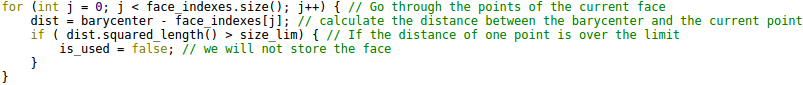
\includegraphics[width=\textwidth]{figures/check_max_dist.png}
  \caption{Vérification de la distance au barycentre}
  \label{fig::check_max_dist}
\end{figure}

Nous utilisons ensuite une autre classe CGAL (\textit{Polyhedron}) qui permet de stocker
une surface en trois dimension. L'avantage de cette classe est qu'elle possède
une méthode permettant d'appliquer une subdivision de Catmull-Clark (voir figure
\ref{fig::subdivide}). Cette subdivision permet de lisser la surface par morceaux
pour l'affichage.
\begin{figure}[ht]
\centering
  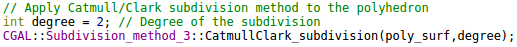
\includegraphics[width=0.8\textwidth]{figures/subdivide.png}
  \caption{Subdivision de Catmull-Clark}
  \label{fig::subdivide}
\end{figure}

\section{Affichage}
\begin{itemize}
  \item .off files $\to$ écriture avec indexation
\end{itemize}

Pour l'affichage des protéines et de l'interface, nous avons choisi les fichiers
\textit{.off} qui permettent de stocker une liste de points (colorés ou non) et
d'indiquer les liens entre chacun de ces points (voir figure \ref{fig::off_file}).

\begin{figure}[ht]
\centering
  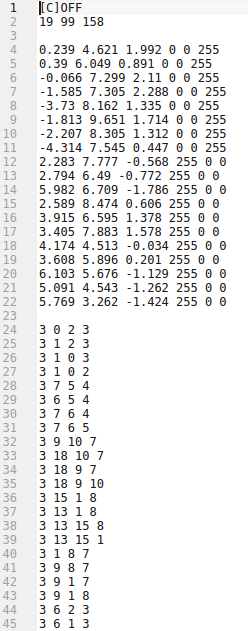
\includegraphics[width=0.3\textwidth]{figures/off_file.png}
  \caption{Exemple de fichier \textit{.off}}
  \label{fig::off_file}
\end{figure}

La première ligne indique le type de fichier (OFF) et la présence ou non de coloration :
[C] si oui un espace vide sinon. La seconde ligne donne, dans cet ordre, le nombre
de points, le nombre de cellules (polyhèdres) et le nombre d'arêtes ce dernier n'étant
pas nécessaire à la lecture du fichier. Dans notre exemple, les lignes 4 à 22 listent
les coordonnées des points et la couleur associée à chacun. La couleur est stockée en RGB
(Rouge, Vert, Bleu) avec des entiers entre 0 et 255 ou des flottants entre 0.0 et 1.0.

Au delà de la ligne 23, les cellules sont listées, avec comme premier entier à chaque
ligne, le nombre de points de la cellule. Comme notre exemple représente une triangulation
de Delaunay, ce nombre vaut 3 car chaque face de la triangulation correspond à un
triangle. A la suite de cet entier viennent les indices des points composant la cellule
(ou la face). Cet indice correspond à la place des coordonnées listées plus haut.


\chapter{Résultats et perspectives}

\section{Résultats}
\begin{itemize}
  \item surface
\end{itemize}

\section{Limitations et problèmes rencontrés}
\begin{itemize}
  \item Compilation
  \item CGAL, structures
\end{itemize}

\section{Perspectives}
\begin{itemize}
  \item Fonctionnalités
\end{itemize}


%% CONCLUSION`
\chapter*{Conclusion}
\addcontentsline{toc}{chapter}{Conclusion}

\cleardoublepage

%%  GLOSSAIRE
%\printnoidxglossary[sort=def] % affichage du glossaire
%\cleardoublepage

%liste des illustrations
\listoffigures
\cleardoublepage

%% BIBLIO
\bibliography{content/ref.bib}
\bibliographystyle{apalike-fr}
\cleardoublepage

% ANNEXES
\appendix % permet d'indiquer que l'on passe dans les annexes, change la numérotation

\part*{Annexes} % nouvelle partie
\addcontentsline{toc}{part}{Annexes} % ajout de l'annexe dans la toc
%\begin{figure}[ht]
\centering
  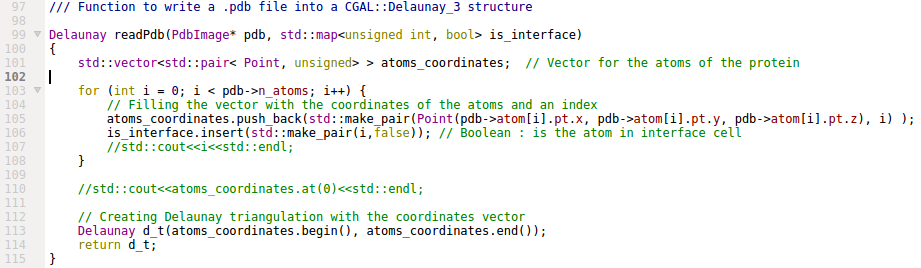
\includegraphics[width=\textwidth]{figures/readPdb.png}
  \caption{Fonction readPdb}
  \label{fig::read_pdb}
\end{figure}

\begin{figure}[ht]
\centering
  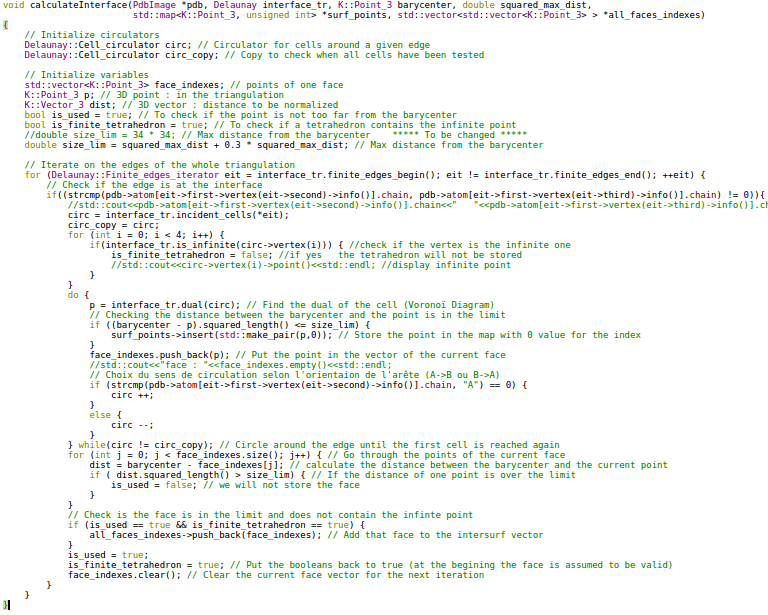
\includegraphics[width=\textwidth]{figures/calculate_interface.png}
  \caption{Fonction calculateInterface}
  \label{fig::calculate_interface}
\end{figure}

\begin{figure}[ht]
\centering
  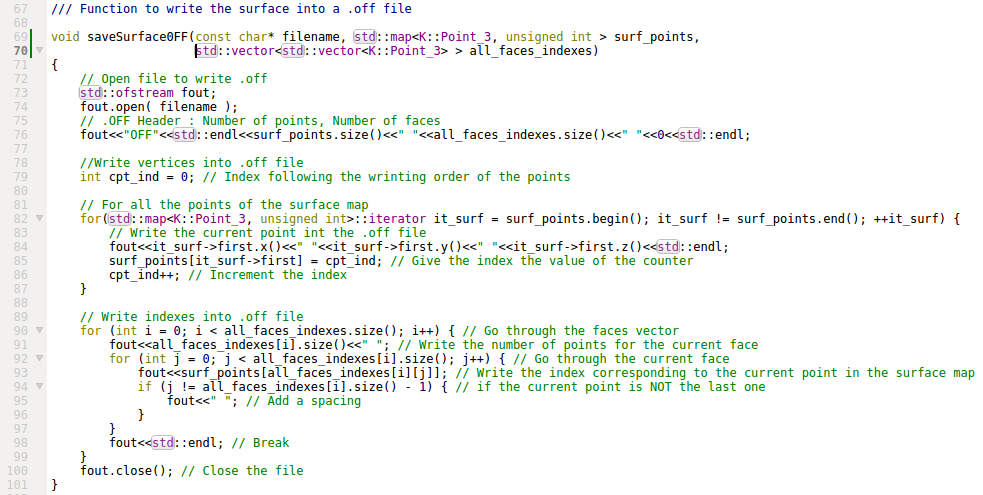
\includegraphics[width=\textwidth]{figures/save_surface_off.png}
  \caption{Fonction saveSurfaceOFF}
  \label{fig::save_surface_off}
\end{figure}

%%  ABSTRACT
%\thispagestyle{empty}

\section*{Résumé}
\addcontentsline{toc}{chapter}{Résumé} % ajout dans toc

{\bf Mots-clés :  }

\section*{Abstract}
\addcontentsline{toc}{chapter}{Abstract} % ajout dans toc

{\bf Keywords : }


\end{document}
